\documentclass{beamer} % Define a classe do documento como Beamer

\usepackage{listings}
\usepackage{xcolor} % necessário para as cores no listings
\usepackage{listings}
\usepackage{xcolor}
\usepackage[percent]{overpic}


\lstset{
	language=R,
	basicstyle=\ttfamily\footnotesize,
	keywordstyle=\color{blue},
	commentstyle=\color{gray},
	stringstyle=\color{red},
	frame=single,
	breaklines=true,
	columns=flexible,
	showstringspaces=false,
	tabsize=2
}

\usetheme{Ilmenau}   
\graphicspath{{figuras/}}  

% Informações do Título
\title{Estudo sobre modelos log-lineares Poisson: \\ Verificação de estimativa pontual e intervalar (tipo link) para as médias}
\author{André Savassi \\ Kenzo Bontempo \\ Márcio Antônio}
\institute{UFMG}
\date{01/10/2025} % Data da apresentação

% CONFIGURAÇÃO PERSONALIZADA DO RODAPÉ
\setbeamertemplate{footline}{
	\leavevmode%
	\hbox{%
		% ESQUERDA: "grupo 2"
		\begin{beamercolorbox}[wd=.33\paperwidth,ht=2.25ex,dp=1ex,left]{author in head/foot}%
			\hspace{0.5cm}\textbf{Grupo 2}%
		\end{beamercolorbox}%
		% CENTRO: "MCCD -2"
		\begin{beamercolorbox}[wd=.34\paperwidth,ht=2.25ex,dp=1ex,center]{title in head/foot}%
			\textbf{MCCD - II}%
		\end{beamercolorbox}%
		% DIREITA: Número da página (opcional)
		\begin{beamercolorbox}[wd=.33\paperwidth,ht=2.25ex,dp=1ex,right]{date in head/foot}%
			\textbf{01/10/2025}
			\insertpagenumber\hspace{0.5cm}%
	\end{beamercolorbox}}%
	\vskip0pt%
}

% Início do Documento
\begin{document}
	
	% Slide de Título
	\begin{frame}
		\titlepage % Gera o slide de título com as informações acima
	\end{frame}
	
	% Sumário (Opcional, mas recomendado)
	\begin{frame}{Sumário}
		\tableofcontents % Gera um sumário automático baseado nas seções
	\end{frame}
	
	% Primeira Seção
	\section{Introdução}
	
	% Slide de Conteúdo
	\begin{frame}{Introdução} % Título do slide vai aqui
		%\framesubtitle{Subtítulo (Opcional)} % Subtítulo opcional
		
		Aqui vai o conteúdo do seu slide.
		
		\begin{itemize}
			\item Este é um item de lista.
			\item<2-> Este item aparece no segundo "clique" (sobreposição).
			\item Outro item importante.
		\end{itemize}
		
		\begin{block}{Título de um Bloco}
			Texto dentro de um bloco destacado.
		\end{block}
	\end{frame}
	
	\section{Distribuições}
	\begin{frame}{Gerando amostras de distribuições - Poisson}
		\subtitle{Distribuição Poisson}
		Primeiramente, iremos amostrar da Distribuição Poisson, que possui a função densidade descrita por:
		$$f(y; \lambda) = \frac{e^{-\lambda} \lambda^y}{y!}, \ y = 0,1,\dots,n$$
		
		Referencia-se que: $\mathbb{E}(Y) = Var(Y) = \lambda$
 		
	\end{frame}
	
	% Segunda Seção e outro Slide

	
\begin{frame}[fragile]{Amostrador Poisson via Transformação Inversa}
	\begin{columns}
		
		\begin{column}{0.85\textwidth}
			\begin{lstlisting}[language=R]
	library(dplyr)
	library(kableExtra)
	rpois_aux <- function(lambda) {
		u <- runif(1, 0, 1)
		i <- 0
		pr <- exp(-lambda)
		Fx = pr
		while (u >= Fx) {
			pr <- pr * lambda / (i + 1)
			Fx <- Fx + pr
			i <- i + 1
		}
		return(i)
	}
	rpoisson <- function(n, lambda) {
		replicate(n, expr = rpois_aux(lambda), simplify = TRUE)
	}		
			\end{lstlisting}
		\end{column}
		
		\begin{column}{0.15\textwidth}
			\href{https://github.com/andresavassi/Trabalho-1---MCCD-II/blob/main/poisson_inversa.R}{\beamergotobutton{Código.R}}
			
			\vspace{0.5cm}

		\end{column}
		
	\end{columns}
\end{frame}

\begin{frame}{Resultados - Poisson Inversa}
	\centering
	\begin{overpic}[width=0.9\textwidth]{tbl_pois_inversa.png}
		% coloca o gráfico por cima
		\put(0,0){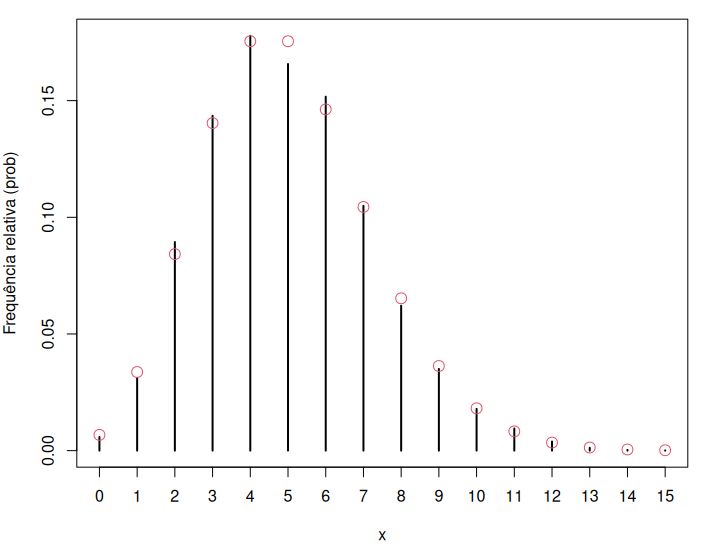
\includegraphics[width=0.6\textwidth]{graf_pois_inversa.png}}
	\end{overpic}
\end{frame}



\begin{frame}[fragile]{Amostrador Poisson via Aceitação/ Rejeição}
	\begin{columns}
		
		\begin{column}{0.85\textwidth}
			\begin{lstlisting}[language=R]
	poisson_ar_1 <- function(lambda, kmax = 30) {
		f_pois <- function(k, lambda) {
			return(exp(-lambda) * lambda^k / factorial(k))
		}	
		fmax <- f_pois(floor(lambda), lambda) 
		repeat {	
			y <- sample(0:kmax, 1)
			fy <- f_pois(y, lambda)		
			gy <- 1 / (kmax + 1)				
			u <- runif(1)
			if (u < fy / (fmax * gy)) {
				return(y)
			}
		}
	}
	poisson_ar <- function(lambda, n = 1000, kmax = 30) {
		replicate(n, poisson_ar_1(lambda, kmax))
	}
			\end{lstlisting}
		\end{column}
		
		\begin{column}{0.15\textwidth}
		\href{https://github.com/andresavassi/Trabalho-1---MCCD-II/blob/main/poisson_ar.R}{\beamergotobutton{Código.R}}
		
		\vspace{0.5cm}
		
		\end{column}
	
	\end{columns}
\end{frame}




	\begin{frame}{Gerando amostras de distribuições - Binomial Negativa}
		Segue que a densidade da distribuição Binomial Negativa é descrita por:
		$$f(y; r,p) = \binom{y-1}{r-1} p^r(1-p)^{y-r}$$
		\ onde $r$ é o total de sucessos e $p$ é a probabilidade desses sucessos.
		Note que $Y \sim BN(r,p)$ possui esperança e variância a seguir:
		$$
		\mathbb{E}(Y) = \frac{r}{p}\ ;\ Var(Y) = \frac{r(1-p)}{p^2}
		$$
		
		
	\end{frame}


	\begin{frame}{Gerando amostras de distribuições - Bell}
		Segue que a densidade da distribuição Bell é descrita por:
		$$
		f(y; \theta) = \frac{\theta e^{e^{\theta} + 1}}{y!} B_Y,\ y = 0, 1, \dots, n; \ \theta > 0
		$$
		
		Onde o termo $B_Y$ corresponde ao número de Bell, dados por:
		
		$$
		B_n= \frac{1}{e} \sum_{k = 0}^{\infty} \frac{k^n}{k!}, \text{iniciando com}\ B_0 = B_1 = 1
		$$
		
		A média e variâncida de $Y \sim Bell(\theta)$ é:
		$$
		\mathbb{E}(Y) = \theta e^{\theta}\ ;\ 
		Var(Y) = \theta(1+\theta)e^{\theta}
		$$
		
	\end{frame}
	
	\begin{frame}[fragile]{Amostrador Bell via Transformação Inversa}
		\begin{columns}
			
			\begin{column}{0.85\textwidth}
				\begin{lstlisting}[language=R]
					n <- 10000
					
					u <- runif(n)
					
					x_inv <- qnorm(u, mean = 0, sd = 1)
					
							
				\end{lstlisting}
			\end{column}
			
			\begin{column}{0.15\textwidth}
				\href{https://github.com/andresavassi/Trabalho-1---MCCD-II/blob/main/bell_inversa.R}{\beamergotobutton{Código.R}}
				
				\vspace{0.5cm}
				
			\end{column}
			
		\end{columns}
	\end{frame}
	
	\begin{frame}{Gráficos - Bell Inversa}
	\begin{figure}[h]
		\centering
		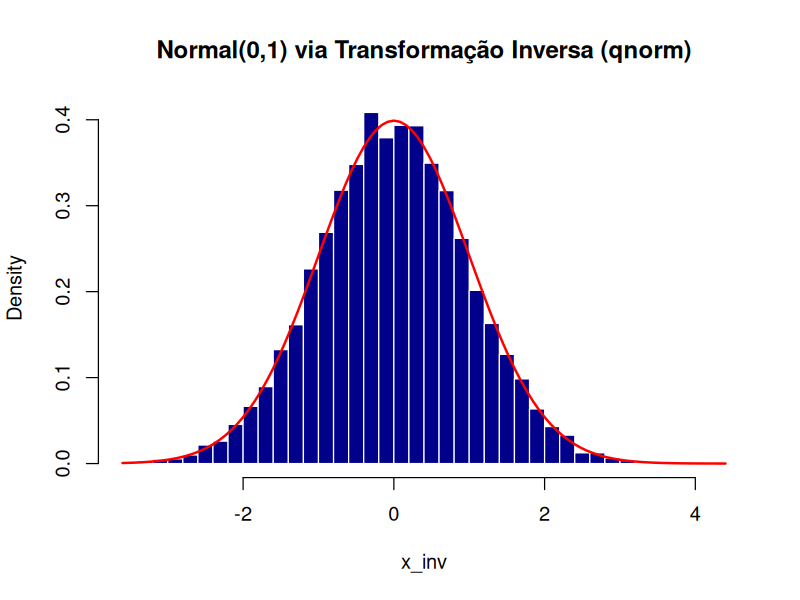
\includegraphics[width=0.8\textwidth]{graf_bell_inv.png}
	\end{figure}
\end{frame}

	\begin{frame}[fragile]{Amostrador Bell via Box Muller}
		\begin{columns}
			
			\begin{column}{0.85\textwidth}
				\begin{lstlisting}[language=R]
					n <- 10000
					
					u1 <- runif(n)
					u2 <- runif(n)
					
					z1 <- sqrt(-2 * log(u1)) * cos(2 * pi * u2)
					z2 <- sqrt(-2 * log(u1)) * sin(2 * pi * u2)
					
					x_bm <- c(z1, z2)
				\end{lstlisting}
			\end{column}
			
			\begin{column}{0.15\textwidth}
				\href{https://github.com/andresavassi/Trabalho-1---MCCD-II/blob/main/bell_bm.R}{\beamergotobutton{Código.R}}
				
				\vspace{0.5cm}
				
			\end{column}
			
		\end{columns}
	\end{frame}
	
	\begin{frame}{Gráficos - Bell Box Muller}
		\begin{figure}[h]
			\centering
			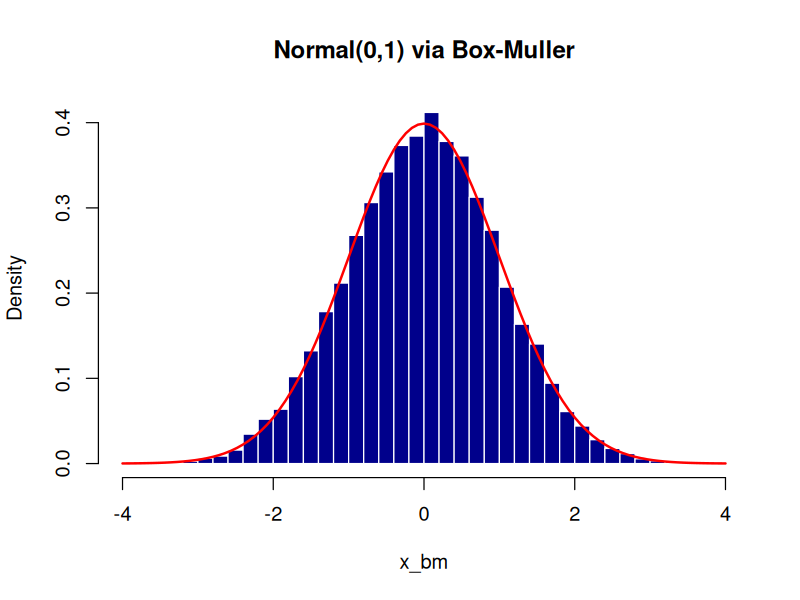
\includegraphics[width=0.8\textwidth]{graf_bell_bm.png}
		\end{figure}
	\end{frame}
	

\section{Implementação}
	


\end{document}
